\documentclass[a4paper,12pt]{report}
\usepackage[serie,niveau={1MA1},nfiche={}, annee={Emilie-Gourd, 2024--2025}, auteur={ns},theme={Série 10}]{packages/bandeaux}
\usepackage{packages/boites}
\usepackage{packages/fontes}
\usepackage{packages/courslatex}

\begin{document}
{\bfseries Lundi $\longrightarrow$ ex. 1,2,3,4  \hfill Jeudi $\longrightarrow$ ex. 5,6,7,8}

\textLigne{Exercices}
\begin{exo}[2]
En utilisant la méthode de complétion du carré, résoudre dans $\mathbb{R}$ les équations suivantes~:
\begin{tasks}(2)
\task $x^2-4 x-1=0$
\task $4 x^2+12 x+5=0$
\task $x^2-6 x-11=0$
%(*) f) $2 x^2-2 x-1=0$
\task $x^2+4 x+6=0$
%(*) g) $15 x^2-23 x-28=0$
\task $x^2+x-1=0$
\task $25 x^2+30 x+2=0$
\end{tasks}
\end{exo}
\begin{exo}[2]
La somme des carrés de trois nombres entiers consécutifs dépasse de $288$ la somme des carrés des deux nombres entiers précédents. Quels sont ces cinq nombres~?
\end{exo}
\begin{exo}[1]
	Trouver deux nombres dont la différence et le produit valent 1.
\end{exo}
\begin{exo}[2]
Un nombre est le produit de trois entiers consécutifs. Si l'on divise ce nombre successivement par chacun des trois entiers, la somme des quotients ainsi obtenus est de $767$.
De quel nombre s'agit-il?
\end{exo}
\begin{exo}[2]
	\begin{tasks}
\task Écrire une équation du troisième degré dont la solution est: $S=\{-3 ; 5 ; 6\}$.
\task Écrire toutes les équations du troisième degré ayant comme solution: $S=\{0 ; 5\}$, et dont le coefficient du terme de degré 3 est 4 .
\task Écrire une équation du plus petit degré possible et ayant comme solution : $S=\left\{0 ;-2 ; \frac{1}{2} ; 5\right\}$.
\task Écrire une équation du deuxième degré dont la solution est : $S=\varnothing$.
	\end{tasks}
\end{exo}
\begin{exo}[1]	
Les deux côtés d'un rectangle ont $6$ mètres de différence. Trouver ses dimensions sachant que son aire est de $9 \mathrm{~m}^2$.
\end{exo}


\begin{exo}[2]
La figure ci-dessous est formée de trois carrés.

\hfill
\begin{minipage}{0.4\textwidth}{
\vspace{0pt}
Que doit mesurer le côté du petit carré pour que la partie ombrée ait une surface triple de la partie blanche~?
}
\end{minipage}
\hfill
\begin{minipage}{0.4\textwidth}{
\vspace{0pt}
\begin{tikzpicture}[scale=1.5]
    \tkzDefPoint[label=below:{}](-2,2){A}
    \tkzDefPoint[label=right:{}](-2,0.5){B}
    \tkzDefPoint[label=above:{}](-0.5,0.5){C}
    \tkzDefPoint[label=above:{}](-0.5,2){D}

    \tkzDefPoint[label=above:{}](-2,0){E}
    \tkzDefPoint[label=above:{}](-0.5,0){F}
    \tkzDefPoint[label=above:{}](0,0){G}
    \tkzDefPoint[label=above:{}](0,0.5){H}
    \tkzDefPoint[label=above:{}](0,2){I}


    \tkzDrawPolygon(A,B,C,D)
    \tkzDrawPolygon(A,E,G,I)
    \tkzDrawPolygon(C,F,G,H)
    \tkzFillPolygon[pattern=north west lines](A,B,C,D)
    \tkzFillPolygon[pattern=north west lines](C,F,G,H)
    \tkzDrawSegment[dashed,dim={$20\text{ cm}$,14pt,right=2mm,midway,font=\footnotesize}](I,G)
	\end{tikzpicture}

}
\end{minipage}
\hfill
\end{exo}
\begin{exo}[1]
Résoudre les équations suivantes dans $\R$:
\begin{tasks}(2)
\task $(x-2)(x-5)=0$
\task $(x+4)(x+6)=0$
\task $(x-3)(7 x-21)=0$
\task $\left(x-\dfrac{1}{4}\right)\left(x+\dfrac{1}{3}\right)\left(\dfrac{2 x}{5}-2\right)=0$
\task $2 x(2 x-1)(3 x+3)=0$
\task $3(2 x-3)\left(5 x-\dfrac{1}{2}\right)=0$
\end{tasks}
\end{exo}
\textLigne{Entraînement individuel}
\begin{exo}
Résoudre dans $\mathbb{R}$ les équations suivantes~:
\begin{tasks}(2)
\task $5 x^2-8 x=0$
\task $4 x^3=9 x$
\task $2 x^3=98 x$
\task $3(x+2)=x(x+2)$
\task $4 x^2+4 x+1=0$
\task $(2 x-6)(x+6)-(4 x+2)(x+6)=0$
\end{tasks}
\end{exo}

\begin{exo}
Factoriser les polynômes suivants dans $\mathbb{R}$ lorsque c'est possible\,:
\begin{tasks}(2)
\task $10 x^2+9 x-9$
\task $-4 x^2+12 x-7$
\task $5 x^2-40 x+76$
\task $x^2-x+2$
\end{tasks}
\end{exo}
\end{document}


